\documentclass{article}

\usepackage{microtype}
\usepackage{graphicx}
\usepackage{booktabs}
\usepackage{hyperref}

\newcommand{\theHalgorithm}{\arabic{algorithm}}

% Blind submission mode (author info stripped automatically)
\usepackage{icml2026}

\usepackage{amsmath, amssymb, amsthm}
\usepackage{xcolor}

% Basic TeX installation lacks Courier metrics; fall back to CM teletype
\renewcommand{\ttdefault}{cmtt}

\icmltitlerunning{Subject-Level Calibration Heterogeneity Across LLM Families and Scales}

\begin{document}

\twocolumn[
  \icmltitle{Subject-Level Calibration Heterogeneity is Stable\\
    Across LLM Families and Scales: A Statistical Audit of MMLU}

  % Author information is automatically hidden in blind-review mode.
  \begin{icmlauthorlist}
    \icmlauthor{Anonymous Author 1}{anon}
    \icmlauthor{Anonymous Author 2}{anon}
  \end{icmlauthorlist}

  \icmlaffiliation{anon}{Anonymous Institution}

  \icmlkeywords{calibration, large language models, MMLU, multilevel models, trustworthy AI}

  \vskip 0.3in
]

\printAffiliationsAndNotice{}

\begin{abstract}
Aggregate calibration metrics for large language models (LLMs) hide structured
heterogeneity in where they are well- and poorly-calibrated. We develop a
statistical audit framework---a multilevel decomposition of question-level
calibration gap variance, isotonic reliability curves per subject, empirical
Bayes shrinkage, and Benjamini--Hochberg FDR correction---and apply it to MMLU
across four instruction-tuned models from two families and three parameter
scales: GPT-4o-mini, Llama-3-8B-Instruct, Qwen-2.5-1.5B-Instruct, and
Qwen-2.5-7B-Instruct. Three findings emerge. (i)~Subject-level ECE rankings are
strongly correlated across all six model pairs (Spearman $\rho \in [0.78,
0.92]$), with cross-family agreement at matched capability stronger than
within-family agreement across scale. (ii)~The same subjects are robustly
worst-calibrated (college-level quantitative STEM, niche factual recall, and
structured ethical/legal reasoning) and robustly best-calibrated
(high-school-level Social Sciences and applied/factual subjects), revealing
specialization level as a meaningful axis of calibration quality. (iii)~Within
the Qwen family, the intercept, between-subject ICC, and entropy coefficient
all change in the direction prior literature on RLHF-induced confidence
saturation \citep{kadavath2022language, nakkiran2025trained} would predict,
consistent with capable instruction-tuned models maintaining near-saturated
confidence even when the option distribution flattens. The stability of
audit findings across models supplies the structural justification for
subject-aware recalibration as in \citet{luo2025pretrained}, and the audit
itself supplies a transferable diagnostic for new models.
\end{abstract}

% ============================================================
\section{Introduction}
% ============================================================

LLMs deployed in high-stakes settings need calibrated confidence as much as
they need accuracy. Most of the calibration literature reports a single
aggregate scalar---ECE \citep{guo2017calibration}, NLL, or related---which is
informative about how much miscalibration there is on average but tells us
nothing about where it concentrates. We ask three questions:

\begin{enumerate}
  \item \textbf{Where is calibration good and bad within a benchmark?}
  \item \textbf{Are these patterns stable across models?}
  \item \textbf{What mechanisms produce the observed heterogeneity?}
\end{enumerate}

Our contribution is a statistical audit framework---multilevel decomposition,
FDR correction, isotonic curves with empirical Bayes shrinkage---that produces
direct answers to these questions, and an application of the framework to four
instruction-tuned LLMs on MMLU \citep{hendrycks2021measuring}. The framework is
diagnostic rather than corrective: \citet{luo2025pretrained} demonstrates that
subject-aware temperature scaling improves on global recalibration; we ask
whether the structural assumption underlying that scoping decision (that
miscalibration patterns are stable enough to be worth scoping over) is
empirically justified.

Prior work has studied LLM calibration mostly at the aggregate level.
\citet{kadavath2022language} showed that token-level logprobs carry a meaningful
calibration signal on multiple-choice tasks and that instruction tuning tends to
degrade it; \citet{xiong2024can} noted calibration degrades on tasks requiring
professional knowledge but did not investigate subject-level structure formally.
\citet{nakkiran2025trained} and \citet{yaldiz2026balancing} document
RLHF-induced confidence saturation at the aggregate level. We bring a formal
statistical audit to the within-benchmark heterogeneity these works describe only
in passing.

% ============================================================
\section{Method}
% ============================================================

\paragraph{Confidence elicitation.}
For each MMLU question we extract token-level log probabilities over
$\{A, B, C, D\}$, softmax-renormalize, and define $c_i$ as the maximum
renormalized probability. The signed calibration gap
$\mathrm{gap}_i = c_i - y_i$ (where $y_i \in \{0, 1\}$ is correctness) is our
primary outcome. GPT-4o-mini is queried via the OpenAI Batch API with
\texttt{top\_logprobs=20}; the open-weight models are run with 4-bit
quantization on a Colab T4 GPU, with the assistant turn pre-filled by ``The
answer is'' to score the next-token position. Test-set accuracies: 0.749, 0.606,
0.536, 0.685 for GPT, Llama, Qwen-1.5B, Qwen-7B respectively.

\paragraph{Multilevel decomposition.}
We fit a three-level mixed-effects model with questions nested in subjects
nested in domains:
\begin{equation}
  \mathrm{gap}_{ijk} = \mu + \mathbf{x}_{ijk}^\top \boldsymbol{\beta}
    + u_k + v_{jk} + \varepsilon_{ijk},
\end{equation}
where $u_k$ is a domain random intercept, $v_{jk}$ a subject-within-domain
intercept, and $\mathbf{x}_{ijk}$ standardized question-level covariates: word
count, max option length, negation indicator, and Shannon entropy of the
A/B/C/D distribution ($H_i = -\sum_k p_{ik} \log p_{ik}$ in nats). Variance
components are estimated by REML; the ICC decomposition reports the share of
total variance at each level.

\paragraph{Calibration curves and ECE.}
For each subject we fit isotonic regression \citep{zadrozny2002transforming}
and an unconstrained Gaussian kernel smoother ($\sigma=1.5$ bins) on
$(c_i, y_i)$, and compute ECE as the 20-bin weighted absolute deviation between
the curve and the diagonal.

\paragraph{Multiple testing.}
For each of 57 subjects we test $H_0$: mean calibration gap $= 0$ via a
one-sample $t$-test on question-level gaps, then apply Benjamini--Hochberg FDR
correction at $\alpha = 0.05$.

% ============================================================
\section{Results}
% ============================================================

\subsection{Variance decomposition (RQ1)}

Table~\ref{tab:icc} reports the ICC decomposition. Across all four models, the
bulk of calibration-gap variance lies at the question level (92.2--98.1\%) and
domain-level variance collapses to zero. Between-subject ICCs differ by nearly
a factor of four---from 1.9\% (Qwen-1.5B) to 7.9\% (GPT-4o-mini), with Qwen-7B
intermediate at 4.9\%. Within the Qwen family, ICC roughly triples as scale
grows from 1.5B to 7B.

\begin{table}[h]
\centering
\small
\caption{Variance decomposition of the calibration gap. Domain-level variance
is estimated at zero for every model; ICC$_\text{subject}$ is the share of
total variance at the subject level.}
\label{tab:icc}
\begin{tabular}{lrrr}
\toprule
Model & $\sigma^2_{\text{subject}}$ & $\sigma^2_\varepsilon$ & ICC$_{\text{subject}}$ \\
\midrule
GPT-4o-mini             & 0.013 & 0.150 & 0.079 \\
Llama-3-8B-Instruct     & 0.004 & 0.190 & 0.020 \\
Qwen-2.5-1.5B-Instruct  & 0.004 & 0.203 & 0.019 \\
Qwen-2.5-7B-Instruct    & 0.009 & 0.177 & 0.049 \\
\bottomrule
\end{tabular}
\end{table}

\subsection{Where calibration succeeds vs.\ fails (RQ1)}

The same subject clusters appear at both extremes of the ECE distribution
across all four models. Four subjects are top-10 most miscalibrated for every
model: \texttt{virology}, \texttt{college\_chemistry}, \texttt{college\_physics},
\texttt{professional\_law}. Top-15 expansion adds
\texttt{college\_mathematics}, \texttt{econometrics},
\texttt{high\_school\_physics}, \texttt{machine\_learning}, and
\texttt{moral\_scenarios}. These cluster into three semantic groups:
college-level quantitative STEM, niche factual recall, and structured
ethical/legal reasoning.

Symmetrically, two subjects are bottom-5 best-calibrated for every model
(\texttt{high\_school\_government\_and\_politics},
\texttt{high\_school\_psychology}); bottom-10 adds
\texttt{high\_school\_us\_history}, \texttt{marketing}, and
\texttt{miscellaneous}. Two patterns:

\begin{itemize}
  \item \textbf{Specialization level matters.} MMLU's high-school-level
    subjects systematically show smaller calibration gaps than their
    college-level counterparts (compare \texttt{high\_school\_psychology} to
    professional and college subjects in similar areas).
  \item \textbf{Domain category matters.} Best-calibrated subjects are
    dominated by Social Sciences and the ``Other'' (applied/factual) MMLU
    category; no STEM subject appears in the bottom-10 intersection across
    models.
\end{itemize}

Figure~\ref{fig:reliability} contrasts top-5 most-miscalibrated and bottom-5
best-calibrated reliability curves for GPT-4o-mini. Curves are masked to the
1st--99th percentile of observed confidence per subject to avoid displaying
isotonic extrapolation in regions with no data. The two panels reveal the
heterogeneity that aggregate ECE conceals: in a single model on a single
benchmark, some subjects sit on the calibration diagonal while others fall
sharply below it.

\begin{figure*}[t]
  \centering
  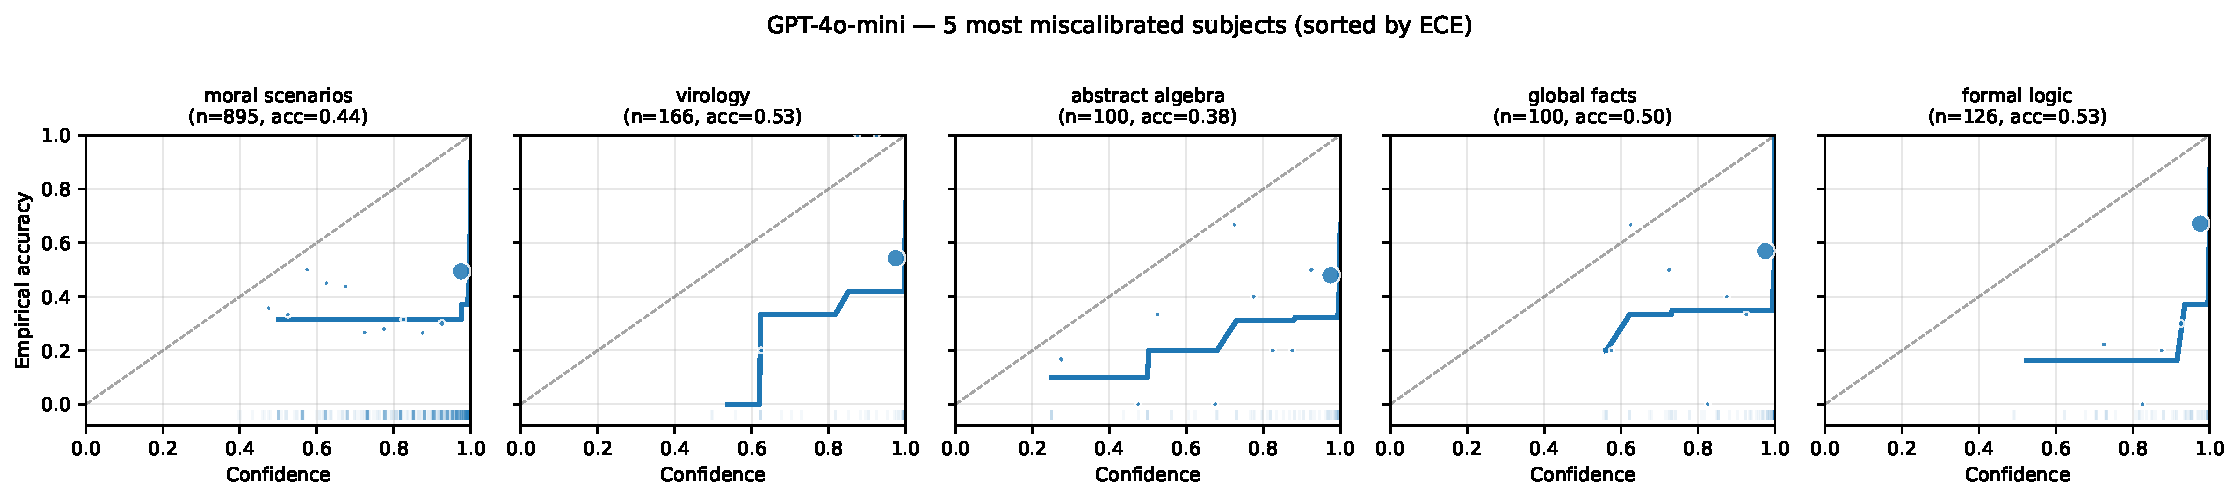
\includegraphics[width=\textwidth]{figures/top5_most_miscalibrated_gpt4o_4m.pdf}
  \vspace{0.5em}
  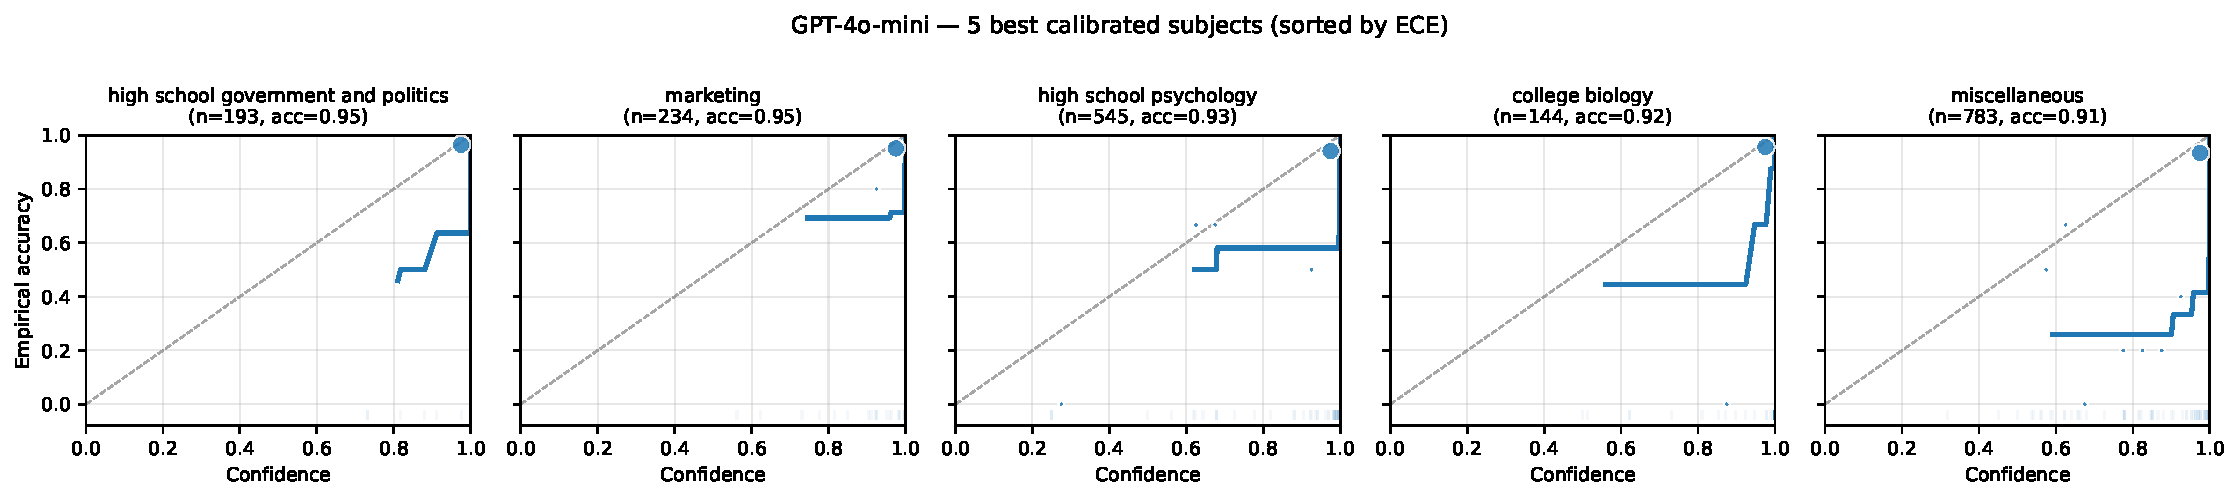
\includegraphics[width=\textwidth]{figures/bottom5_best_calibrated_gpt4o_4m.pdf}
  \caption{GPT-4o-mini reliability curves. \textbf{Top}: five most miscalibrated
  subjects by ECE. \textbf{Bottom}: five best-calibrated subjects. Same
  conventions in both: solid line is isotonic regression, plotted only on
  observed support; markers are 20-bin empirical accuracy sized by bin count;
  dashed line is the calibration diagonal.}
  \label{fig:reliability}
\end{figure*}

\subsection{Cross-model agreement (RQ2)}

Figure~\ref{fig:crossmodel} reports the 4$\times$4 Spearman rank correlation
matrix of subject-level ECE. All six pairwise correlations fall in
$[0.78, 0.92]$. The cross-family GPT-4o-mini vs Qwen-7B pair is the highest
(0.924), exceeding the within-family Qwen scaling correlation (0.849).
Cross-family agreement at matched capability is therefore stronger than
within-family agreement across scale---the strongest evidence in our data
that subject-level miscalibration is a property of the task, not the model.

Bootstrap 95\% CIs (2000 replicates): GPT vs Llama $[0.73, 0.91]$, GPT vs
Qwen-1.5B $[0.64, 0.87]$, GPT vs Qwen-7B $[0.85, 0.96]$, Llama vs Qwen-1.5B
$[0.73, 0.89]$, Llama vs Qwen-7B $[0.80, 0.93]$, Qwen-1.5B vs Qwen-7B
$[0.76, 0.90]$.

\begin{figure}[h]
  \centering
  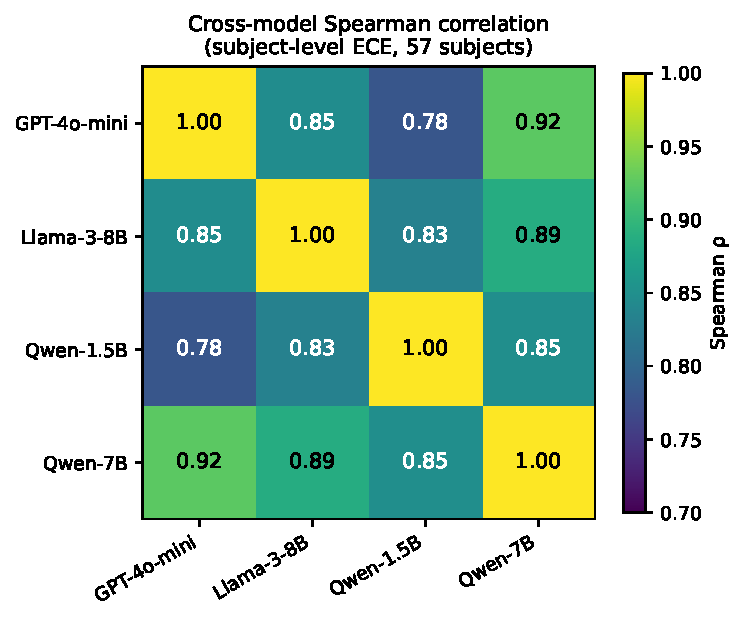
\includegraphics[width=\columnwidth]{figures/cross_model_heatmap_4m.pdf}
  \caption{Spearman rank correlation matrix of subject-level ECE across the
  four models (57 common subjects). All pairwise correlations are between
  0.78 and 0.92.}
  \label{fig:crossmodel}
\end{figure}

\subsection{Mechanism: predictors and within-family scale (RQ3)}

Table~\ref{tab:fixef} reports the fixed effects from the multilevel model.
Intercepts confirm large mean overconfidence (0.157--0.233). Within the Qwen
family, the larger 7B model is more overconfident than the smaller 1.5B
($+49\%$ in the intercept) despite higher accuracy---consistent with
\citet{kadavath2022language} on RLHF-induced confidence inflation.

\begin{table}[h]
\centering
\small
\caption{Fixed effects from the three-level mixed model. Continuous covariates
standardized. Significance: $^{***}p<0.001$, $^{**}p<0.01$, $^*p<0.05$,
$^\dagger p<0.10$.}
\label{tab:fixef}
\begin{tabular}{lrrrr}
\toprule
Predictor & GPT & Llama & Q-1.5B & Q-7B \\
\midrule
Intercept         &  0.196$^{***}$ &  0.197$^{***}$ &  0.157$^{***}$ &  0.233$^{***}$ \\
Word count        &  0.031$^{***}$ & -0.005          &  0.004          &  0.019$^{**}$  \\
Max option len.   &  0.001          & -0.001          & -0.002          & -0.007          \\
Negation          & -0.001          &  0.007          & -0.010          & -0.001          \\
Entropy           &  0.016$^{***}$ &  0.008$^\dagger$ & -0.010$^{*}$    &  0.029$^{***}$ \\
\bottomrule
\end{tabular}
\end{table}

\begin{figure}[h]
  \centering
  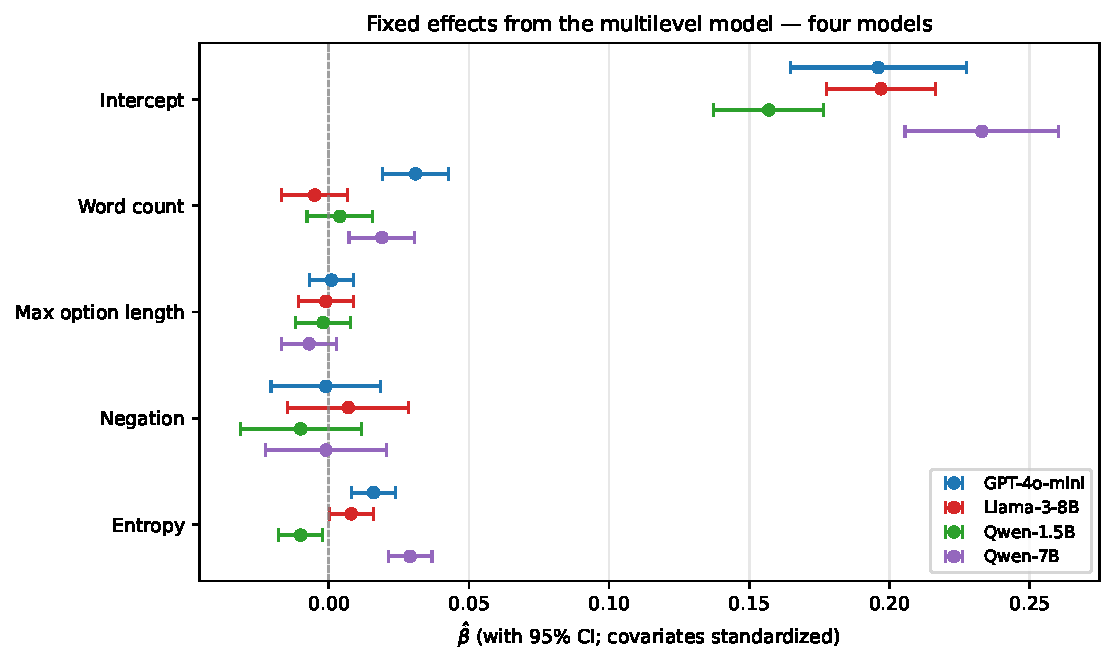
\includegraphics[width=\columnwidth]{figures/coef_plot_4m.pdf}
  \caption{Fixed effect estimates with 95\% confidence intervals across the four
  models. The entropy sign flip (negative for Qwen-1.5B, positive for the other
  three) is the most informative pattern.}
  \label{fig:coef}
\end{figure}

\paragraph{Entropy: a sign flip across capability.}
The most informative predictor is entropy. A naïve prediction is that high
option-distribution entropy should reduce the calibration gap, since top-1
confidence is mechanically lower when probability mass spreads. Yet the
entropy coefficient is positive for GPT-4o-mini ($+0.016$, $p<0.001$) and
Qwen-7B ($+0.029$, $p<0.001$), marginal for Llama, and \emph{negative} for
Qwen-1.5B ($-0.010$, $p=0.018$). Figure~\ref{fig:entropy} traces the mechanism
by partitioning each model's questions into entropy quartiles and plotting
mean confidence (solid) vs.\ mean accuracy (dashed). In three of four models
confidence falls slower than accuracy as entropy rises, widening the gap;
Qwen-1.5B is the only model where the two fall in parallel, exactly the
reason its entropy coefficient is negative.

\begin{figure*}[t]
  \centering
  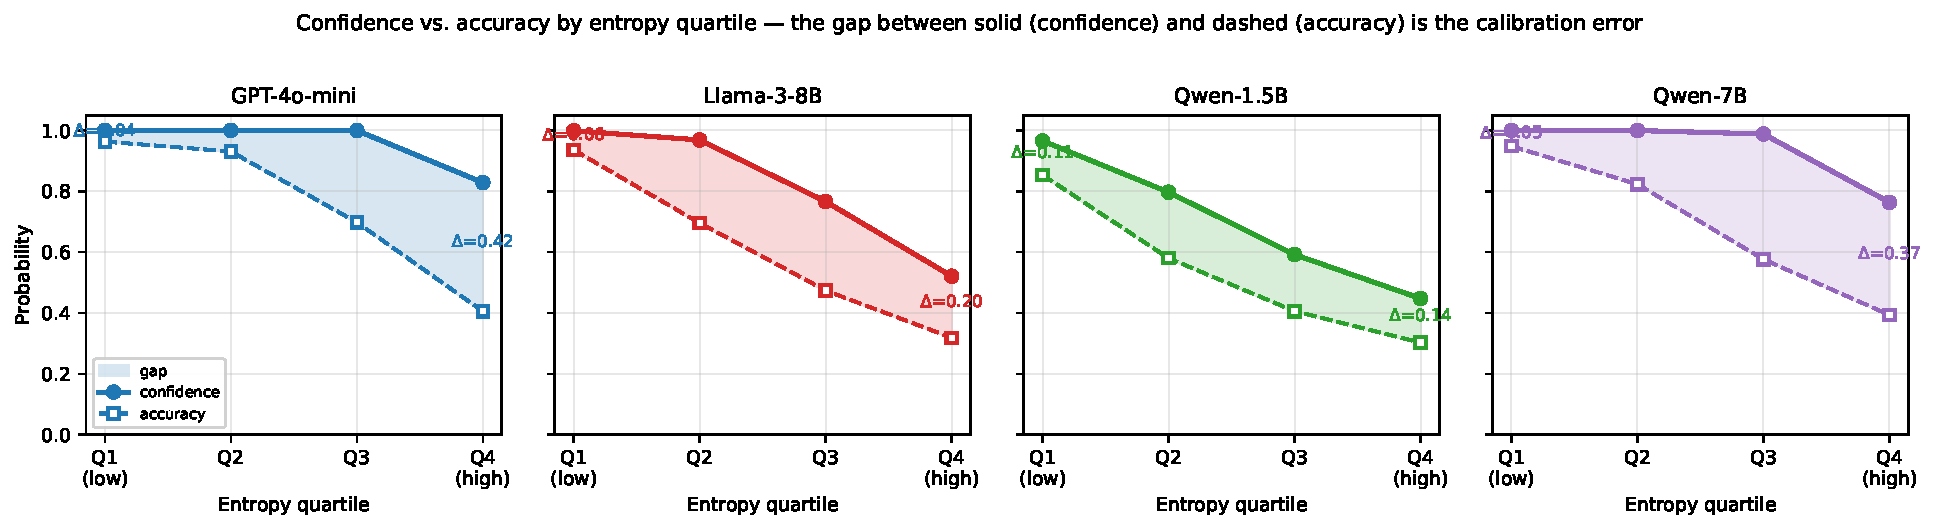
\includegraphics[width=\textwidth]{figures/entropy_mechanism_4m.pdf}
  \caption{Confidence (solid) and accuracy (dashed) by entropy quartile per
  model. Shaded area is the calibration gap. Three of four models show
  confidence falling more slowly than accuracy as entropy rises; only
  Qwen-1.5B shows the two falling in parallel.}
  \label{fig:entropy}
\end{figure*}

This pattern aligns with prior aggregate findings on RLHF and confidence
\citep{kadavath2022language, nakkiran2025trained, yaldiz2026balancing}---more
capable, more aggressively-aligned models maintain confidence near saturation
even when the option distribution flattens. We are cautious about extending
this further: the negative-coefficient finding rests on a single small
checkpoint (Qwen-1.5B), and the variation is between models rather than within
a controlled scaling sweep. The marginal pattern is consistent with the
literature; a stronger causal claim would require additional small or base
models.

\subsection{FDR-corrected rankings and sensitivity}

At $\alpha = 0.05$, all 57 subjects are FDR-rejected for GPT-4o-mini, Llama,
and Qwen-7B; for Qwen-1.5B, 54/57 are rejected. The three subjects that fail
to reject for Qwen-1.5B are
\texttt{high\_school\_government\_and\_politics} ($p_\text{adj}=0.37$),
\texttt{sociology} ($p_\text{adj}=0.24$), and \texttt{us\_foreign\_policy}
($p_\text{adj}=0.14$)---all in Social Sciences and overlapping the
robust well-calibrated set. The substantive finding is the magnitude of
heterogeneity: per-model gap ranges span 6.2--13.9$\times$ from the
best-calibrated to the worst-calibrated subject.

Figure~\ref{fig:meangap} shows all 57 subjects sorted by mean calibration gap
for GPT-4o-mini, with FDR-rejected subjects highlighted. The key takeaway is the
magnitude of heterogeneity: gap ranges span 6.2--13.9$\times$ from the
best-calibrated to the worst-calibrated subject across models.

\begin{figure*}[t]
  \centering
  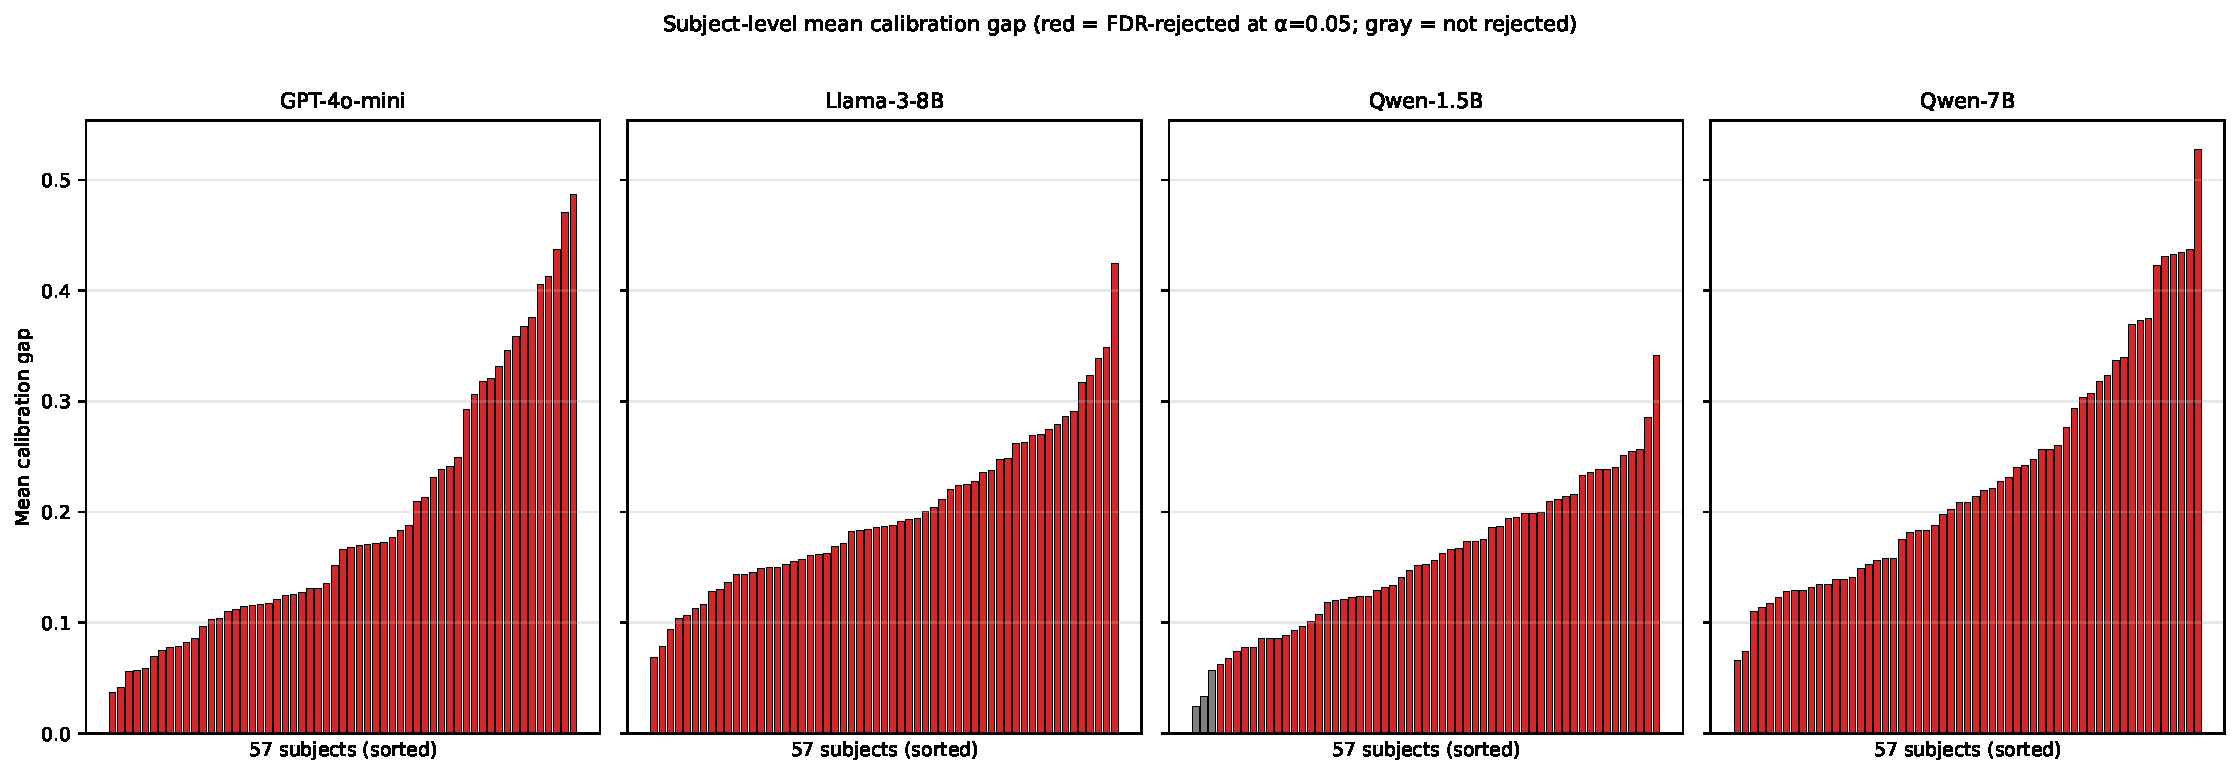
\includegraphics[width=\textwidth]{figures/subject_mean_gap_4m.pdf}
  \caption{Mean calibration gap per subject, sorted ascending, for all four
  models. Red bars are FDR-rejected at $\alpha=0.05$; gray bars are not. Three
  of four models reject all 57 subjects; Qwen-1.5B rejects 54 of 57.}
  \label{fig:meangap}
\end{figure*}

Sensitivity-analysis conclusions extend uniformly: ECE rankings are stable
across bin counts (Spearman $\geq 0.97$ vs.\ 20-bin baseline), proper-scoring
NLCS rankings track ECE rankings (Spearman $\geq 0.85$), and two-level vs.\
three-level ICC estimates are numerically identical (consistent with
$\sigma^2_\text{domain}=0$).

% ============================================================
\section{Discussion}
% ============================================================

\paragraph{What the audit recovers.} Aggregate ECE understates structured
heterogeneity that is real (FDR-rejected, robust to bin choice, robust to
proper-scoring metrics), task-driven (correlated across families and scales),
and aligned with intuitive content axes (specialization level, domain
category). The robust well-calibrated set (high-school-level Social Sciences
and applied subjects) and the robust poorly-calibrated set (college-level
quantitative STEM, niche factual recall, structured reasoning) appear in every
model we examined.

\paragraph{Implications for recalibration.} Stable cross-model targets
provide the structural justification for choosing subject-aware recalibration
scoping over global recalibration. We do not re-fit the corrections themselves
(those would still be model-specific): \citet{luo2025pretrained} demonstrates
the operational arm directly. Our framework supplies the diagnostic upstream:
when miscalibration patterns are this stable across very different training
pipelines, scoping a correction at the subject level is the structurally
appropriate choice. The audit findings also provide a transferable diagnostic:
the robustly worst-calibrated subjects we identify can flag miscalibration on
new models before deployment.

\paragraph{Limitations.}
The within-family scale comparison rests on two checkpoints (Qwen-1.5B and
Qwen-7B); the entropy-coefficient sign flip rests on Qwen-1.5B alone.
Replication with additional scale points (Qwen-2.5-14B) and additional small
or base-model checkpoints (Llama-3-8B-base) would test whether the trend is
monotonic. Cross-family generalization would benefit from a third family
(Mistral-7B or Gemma-2-9B) at matched scale. 4-bit quantization affects three
of the four models studied and may attenuate confidence; Qwen-1.5B's
test-set accuracy is below its published full-precision figure, and its
anomalous entropy coefficient and FDR-robustness gap may be partly artifacts
of quantization. Findings are specific to MMLU's four-choice format and do
not directly extend to open-ended generation.

\paragraph{Future work.} Three extensions are most direct: (i) a continuous
within-family scaling sweep, e.g., Qwen-2.5 \{1.5B, 7B, 14B\}, fitting
intercept and entropy coefficient as functions of scale; (ii) a third model
family at matched scale, strengthening the cross-family claim from two
families to three; (iii) replication on harder benchmarks (MMLU-Pro) to test
whether the high-school vs.\ college calibration gap persists at higher
difficulty.

% ============================================================
\section{Conclusion}
% ============================================================

Subject-level calibration heterogeneity in LLMs is real, large, and stable.
Applied/factual high-school subjects are reliably well-calibrated across all
models we examined; college-level technical content, niche factual recall, and
structured ethical/legal reasoning are reliably poorly calibrated. Subject-level
ECE rankings are highly correlated across all six model pairs
($\rho \in [0.78, 0.92]$), including cross-family pairs at matched capability,
establishing these patterns as properties of the task rather than any particular
training pipeline. The audit supplies the structural justification for
subject-aware recalibration scoping and a transferable diagnostic for flagging
miscalibration on new models before deployment.

% ============================================================
\bibliographystyle{icml2026}
\bibliography{references}
% ============================================================

\end{document}
